\chapter{留数定理}

\begin{introduction}
    \item 留数
    \item 留数定理的应用
\end{introduction}

\section{留数}
    \subsection{留数的定义和留数定理}
        设$z=z_0$为函数$f(z)$的孤立奇点,将$f(z)$在$z_0$的去心领域上展开为$Laurent$级数
        \begin{align*}
            f(z)=\sum_{n=-\infty}^{\infty}a_n(z-z_0)^n\equiv \sum_{n=0}^{\infty}a_n(z-z_0)^n + \frac{b_1}{z-z_0}+\frac{b_2}{z-z_0}+\cdots
        \end{align*}
        其中
        \begin{align*}
            a_n=\frac1{2\pi i}\oint_C \frac{f(\xi)d\xi}{(\xi - z_0)^{n+1}},\ b_n=\frac1{2\pi i}\oint_C f(\xi)(\xi - z_0)^{n-1}d\xi
        \end{align*}
        取其中的
        \begin{align}
            \label{eq:residue}
            b_1=\frac1{2\pi i}\oint_C f(\xi)d\xi
        \end{align}
        我们就将$b_1$称为函数$f(z)$在点$z_0$处的留数,记作$\mathrm{Res} f(z_0)$.

        式\ref{eq:residue}又可写作
        \begin{align*}
            \oint_C f(z)dz=2\pi i \mathrm{Res} f(z_0)
        \end{align*}

        \begin{theorem}[留数定理]\label{thm:residue_theorem}
            令$C$为正向封闭曲线,函数$f$在$C$上连续解析,且$f$在$C$内只有有限个孤立奇点$z_1,\,z_2,\,\cdots,\,z_m$.则
            \begin{align*}
                \oint_C f(z)dz=2\pi i\sum_{k=1}^{m}\mathrm{Res}f(z_k)
            \end{align*}
        \end{theorem}

        仔细观察可能会发现,留数定理和$CIF$(定理\ref{thm:cauchy_integral_formula})有十分甚至九分相似,实际上留数定理就是通过$CIF$及其引理小圆弧引理(引理\ref{lem:small_arc_lemma})证明来的,下一节中给出的求留数的方法使得留数定理在计算某些形式的积分时有奇效,非常的方便,非常的简单.

    \subsection{留数的计算}
        对函数进行$Laurent$展开后直接取$(z-z_0)^{-1}$项的系数是求留数最通用的方法,但是这种方法德川用了都喊牡蛎,由以下命题我们可以非常简便地求出留数.

        \begin{proposition}\label{prop:poles_of_rational_function}
            一个在有限域内所有奇点都是极点的复变函数是一个有理函数($rational function$).
        \end{proposition}

        补充一下有理函数的定义.

        \begin{definition}[有理函数]\label{def:rational_function}
            形如$f(z)=P(z)/Q(z)$的函数被称作有理函数,其中$P(z)$和$Q(z)$均是关于$z$的多项式.
        \end{definition}
        
        关于命题\ref{prop:poles_of_rational_function}的证明可以参考Sadri Hassani的$Mathematical Physics PartI, p343$.

        由命题\ref{prop:poles_of_rational_function},对于一个有$m$阶奇点$z=z_0$的复变函数$f$,另一个函数$g(z)\equiv (z-z_0)^mf(z)$在$z_0$处解析.由此,对于包含$z_0$的封闭路径$C$,有
        \begin{align*}
            Res[f(z_0)]=\frac1{2\pi i}\oint_{C}f(z)dz=\frac1{2\pi i}\oint_C \frac{g(z)dz}{(z-z_0)^m}=\frac{g^{(m-1)}(z_0)}{(m-1)!}
        \end{align*}

        我们可以给出留数的计算定理.

        \begin{theorem}
            复函数$f$有$m$阶极点$z_0$,则
            \begin{align*}
                Res\left[f(z_0)\right]=\frac1{(m-1)!}\lim_{z\to z_0}\frac{d^{m-1}}{dz^{m-1}}\left[(z-z_0)^mf(z)\right].
            \end{align*}
        \end{theorem}

        当$m=1$时
        \begin{align*}
            Res\left[f(z_0)\right]=\lim_{z\to z_0}\left[(z-z_0)f(z)\right].
        \end{align*}

        \begin{remark}
            若要求$\infty$处的留数,则令$t=1/z$,求函数$g(t)=f(1/t)$在$0$处的留数.
        \end{remark}

\section{留数定理的应用}
    为了将留数定理应用到实变函数积分上,我们先给出$Jordan$引理.
    \begin{lemma}[$Jordan$引理]\label{lem:Jordan_lemma}
        设$C_R$为以$R$为半径,坐标原点为圆心的上半圆(位于第一二象限),$\alpha$为任意实数.则当$f$在$z\to\infty$时一致趋于$0$的速度大于$1/|z|$时有
        \begin{align*}
            \lim_{R\to\infty}I_R\equiv \lim_{R\to\infty}\int_{C_R}e^{i\alpha z}f(z)dz=0.
        \end{align*}

    \end{lemma}

    \begin{remark}
        注意$Jordan$引理对$\alpha =0$的情况同样适用,并且我们一般都是这样取的.
    \end{remark}

    通过$Jordan$引理我们就能很方便地把无穷实变积分转化为封闭区线上的复变积分,进而使用留数定理求得积分值.

    \subsection{有理函数的积分}

    有理函数由定义\ref{def:rational_function}给出,我们可以使用留数定理求解有理函数的积分.
    \begin{align*}
        I_1=\int_{-\infty}^{\infty}\frac{p(x)}{q(x)}dx.
    \end{align*}

    我们可以将$I_1$使用复变函数写为
    \begin{align*}
        I_1=\lim_{R\to\infty}\int_{-R}^{R}\frac{p(x)}{q(x)}dx=\lim_{R\to\infty}\int_{C_x}\frac{p(z)}{q(z)}dz.
    \end{align*}

    $C_x$是在实轴上由$-R$到$R$的线段,由$Jordan$引理,我们可以在$C_x$的基础上添加一个半径为$R$的上半圆而不影响积分值,组成闭合曲线$C$.于是我们有
    \begin{align*}
        I_1=\lim_{R\to\infty}\oint_{C}\frac{p(z)}{q(z)}dz=2\pi i\sum_{j=1}^{k}Res\left[\frac{p(z_j)}{q(z_j)}\right].
    \end{align*}

    其中$\left\{z_j\right\}_{j=1}^{k}$为复变函数$p(z)/q(z)$在上半平面有限域内的极点,也就是多项式函数$q(z)$的零点.

    \subsection{含三角函数的有理函数的积分}

    此类积分长这样
    \begin{align*}
        \int_{-\infty}^{\infty}\frac{p(x)}{q(x)}\cos{ax}dx,\ \int_{-\infty}^{\infty}\frac{p(x)}{q(x)}\sin{ax}dx.
    \end{align*}

    这里要求多项式函数$q(x)$没有实数零点,我们可以看到,上面的两个积分分别是如下积分的实部和虚部.
    \begin{align*}
        \int_{-\infty}^{\infty}\frac{p(x)}{q(x)}e^{iax}dx.
    \end{align*}

    后面的操作就和上面的一样了,使用复变量$z$替代$x$后通过留数定理即可求得积分值,注意对最后的结果取实部或虚部.

    \subsection{有理三角函数的积分}

    第三类积分中只涉及三角函数,形如
    \begin{align*}
        \int_{0}^{2\pi}F(\sin{\theta},\cos{\theta})d\theta.
    \end{align*}

    其中函数$F$一般为有理函数,对变量$\theta$进行变换$z=e^{i\theta},\ e^{-i\theta}=1/z$,我们有
    \begin{align*}
        I_3=\oint_{C}F\left(\frac{z-1/z}{2i}, \frac{z+1/z}{2}\right)\frac{dz}{iz}
    \end{align*}

    随后即可使用留数定理处理.

    \subsection{含多值函数的积分}

        这里直接上作业册留数定理中的最后一题(据称这题曾是考试题,可以多留意一下).
        \begin{example}\label{ex:multi_valued}
            \begin{align*}
            \text{计算积分:}\int_0^\infty \frac{x^{a-1}}{1-x}dx.
            \end{align*}
        \end{example}

        \begin{figure}
            \centering
            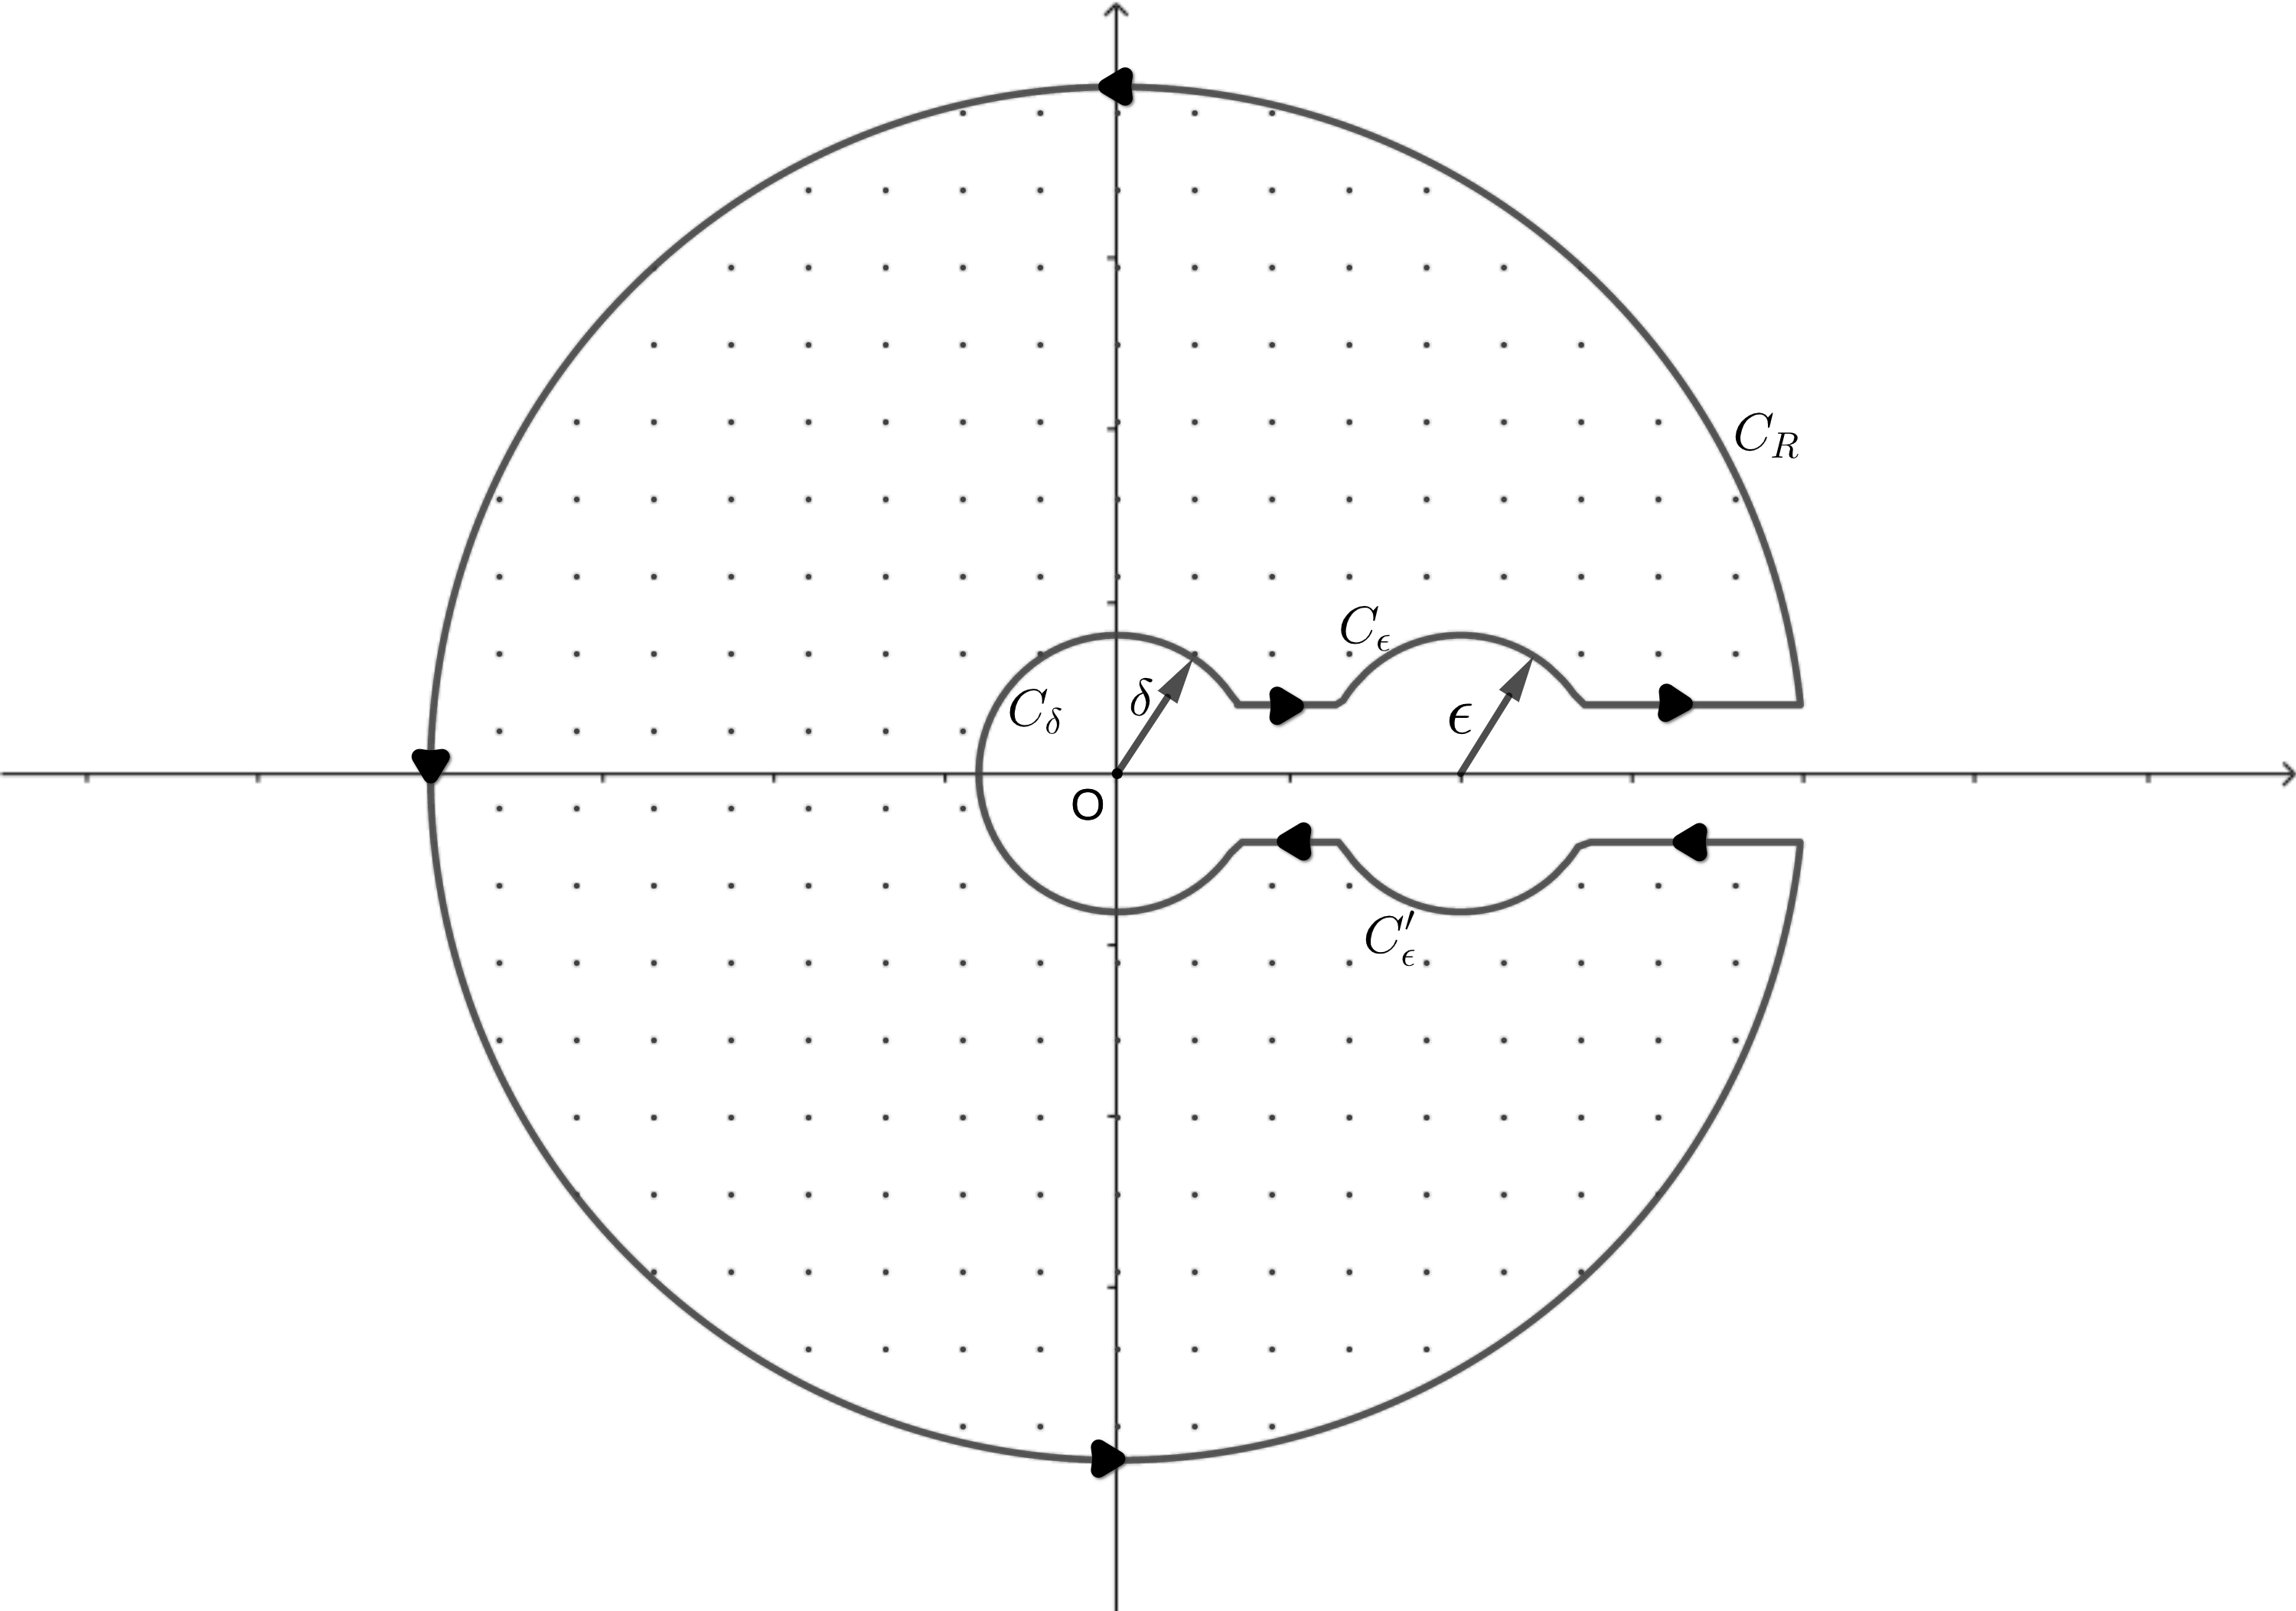
\includegraphics[width=0.5\textwidth]{MultivalueIntPath.png}
            \caption{例\ref{ex:multi_valued}积分路径}
            \label{fig:MultivalueIntPath}
        \end{figure}

        \begin{solution}
            首先取被积函数$f(z)=z^{a-1}/(1-z)$.被积函数$f(z)$有两个枝点$z=0,\ z=\infty$,所以我们取割线$0\to +\infty$沿$x$轴.同时$f(z)$有一阶奇点$z=1$,我们如图\ref{fig:MultivalueIntPath}取积分环路.此时实积分被转化为沿环路的复积分.

            \begin{align}
                \begin{split}\label{eq:multi_valued_integral}
                    I&=\oint_C f(z)dz\\ &=\int_{C_R}f(z)dz+\int_{C_\delta}f(z)dz+\int_{C_\epsilon}f(z)dz+\int_{C'_\epsilon}f(z)dz\\ &+\int_{\delta}^{1-\epsilon}f(x)dx+\int_{1+\epsilon}^{R}f(x)dx+\int_{Re^{2\pi i}}^{(1+\epsilon')e^{2\pi i}}f(x)dx+\int_{(1-\epsilon')e^{2\pi i}}^{\delta e^{2\pi i}}f(x)dx\\ &=0.
                \end{split}
            \end{align}

            由大圆弧引理\ref{lem:large_arc_lemma}
            \begin{align*}
                \lim_{R\to\infty}f(z)dz=i\cdot\lim_{z\to\infty}zf(z)\cdot 2\pi=0.
            \end{align*}

            由小圆弧引理\ref{lem:small_arc_lemma}
            \begin{align*}
                &\lim_{\epsilon\to0}\int_{C_\epsilon}f(z)dz=i\cdot\lim_{z\to1}(z-1)f(z)\cdot\pi=-\pi i.\\
                &\lim_{\epsilon'\to0}\int_{C_{\epsilon'}}f(z)dz=i\cdot\lim_{z\to e^{2\pi i}}(z-1)f(z)\cdot\pi=-\pi ie^{2(a-1)\pi i}.\\
                &\lim_{\delta\to0}\int_{C_\delta}f(z)dz=i\cdot\lim_{z\to0}zf(z)\cdot\pi=0.
            \end{align*}

            同时又有
            \begin{align*}
                &\lim_{\substack{\delta\to0 \\ \epsilon\to0}}\int_{\delta}^{1-\epsilon}f(x)dx+\lim_{\substack{\epsilon \to0\\ R\to\infty}}\int_{1+\epsilon}^{R}f(x)dx=\int_{0}^{\infty}f(x)dx.\\
                &\lim_{\substack{\epsilon' \to0 \\ R\to\infty}}\int_{Re^{2\pi i}}^{(1+\epsilon')e^{2\pi i}}f(x)dx+\lim_{\substack{\epsilon' \to0 \\ \delta\to0}}\int_{(1-\epsilon')e^{2\pi i}}^{\delta e^{2\pi i}}f(x)dx=e^{2a\pi i}\int_{\infty}^{0}f(x)dx.
            \end{align*}

            于是式\ref{eq:multi_valued_integral}被我们转化为
            \begin{align*}
                (1-e^{2a\pi i})\int_{0}^{\infty}\frac{x^{a-1}}{1-x}dx=\pi i+\pi ie^{2(a-1)\pi i}.
            \end{align*}

            解得
            \begin{align*}
                \int_{0}^{\infty}\frac{x^{a-1}}{1-x}dx=\pi \cos{a\pi}.
            \end{align*}


        \end{solution}
